\chapter{Technical Risk Assessment}
\label{chapter:TechRiskAnalysis}
Now that the final design (C2.1: Rotating Wing) was chosen during the trade-off, a risk analysis is conducted to further assess the design. In this chapter, the risks are identified and quantified.
Afterwards, mitigation strategies and contingency plans are implemented, concluding with the risk maps. In order to correctly identify and quantify risks, the same risk metrics of 1--5 for likelihood and impact are used as in previous reports~\cite{baselinerepo,ProjectPlan}. These are presented in \Cref{tab:likelihood_metrics,tab:impact_metrics}. By using these metrics, each identified risk is quantifiable, enabling performance of the risk analysis, which can be seen in \Cref{tab:tech_risk_analysis}. Each risk is described with its impact quantified. The risk factor is calculated by multiplying likelihood and impact, then dividing by five. This generates an unmitigated risk map (see \Cref{fig:Risk_map}), useful as a risk benchmark.

\begin{table}[ht]
    \centering
    \begin{minipage}{0.5\textwidth}
        \centering
        \caption{Likelihood metrics}
        \label{tab:likelihood_metrics}
        \begin{tabular}{ccc}
            \toprule
            \textbf{Likelihood} & \textbf{Description} & \textbf{Probability}         \\ \midrule
            5          & Very High   & $P$ $\geq$ 0.7         \\
            4          & High        & 0.5 $\leq$ $P$ < 0.7 \\
            3          & Moderate    & 0.3 $\leq$ $P$ < 0.5  \\
            2          & Low         & 0.05 $\leq$ $P$ < 0.3 \\
            1          & Very Low    &  $P$ < 0.05          \\ \bottomrule
        \end{tabular}
    \end{minipage}\hfill
    \begin{minipage}{0.5\textwidth}
        \centering
        \caption{Impact metrics}
        \label{tab:impact_metrics}
        \begin{tabular}{cc}
            \toprule
            \textbf{Impact} & \textbf{Description}  \\ \midrule
            5      & Catastrophic \\
            4      & Critical     \\
            3      & Marginal     \\
            2      & Acceptable   \\
            1      & Negligible   \\ \bottomrule
        \end{tabular}
    \end{minipage}
\end{table}

\begin{table}[H]
\caption{Technical risk analysis. ID structure: category - period - chronological numbering}
\label{tab:tech_risk_analysis}
\resizebox{\textwidth}{!}{%
\begin{tabular}{lcllccS[table-format=1.1,round-mode=places,round-precision=1,round-pad=true]}
\toprule
\multirow{2}{*}{\textbf{Risk ID}}   & \multirow{2}{*}{\textbf{Period}}      & \multirow{2}{*}{\textbf{Risk Description}}                                 & \multirow{2}{*}{\textbf{Impact Description}}                                            & \multicolumn{3}{c}{\textbf{Unmitigated Risk}}\\
          &             &                                                  &                                                               & \textbf{Likelihood}      & \textbf{Impact} & \textbf{Risk} \\ \midrule
TR-DES-1  & Design      & Deficient thrust generation                      & Unable to take-off                                            & 2                & 5      & \riskcolor{2}    \\
TR-DES-2  & Design      & Unavailable Additive Manufacturing facilities    & No 3D-model, so no visualisation of the design                & 2                & 3      & \riskcolor{1.2}  \\
PR-PRD-1  & Production  & Components too complex to manufacture            & Part cannot be manufactured, thus an unfeasible design        & 2                & 4      & \riskcolor{1.6}  \\
PR-PRD-2  & Production  & Subcontractor does not meet deadlines            & Delay of construction of the vehicle, testing and operations  & 3                & 4      & \riskcolor{2.4}  \\
PR-PRD-3  & Production  & Subcontractor's part not meeting requirements    & Failure of components results into a delay of production      & 1                & 5      & \riskcolor{1}    \\
PR-PRD-4  & Production  & Part manufacturing costs go over-budget          & Less budget for other segments or a budget short Ance         & 3                & 3      & \riskcolor{1.8}  \\
PR-PRD-5  & Production  & The required material is unavailable             & Delay of production                                           & 3                & 4      & \riskcolor{2.4}  \\
PR-PRD-6  & Production  & Increase in  material costs                      & Extra induced costs                                           & 4                & 3      & \riskcolor{2.4}  \\
LR- TST-1 & Testing     & eVTOL is damaged during transportation           & Extra time and budget needed to repair/redesign the eVTOL     & 1                & 4      & \riskcolor{0.8}  \\
LR- TST-2 & Testing     & Unavailable testing facility                     & Delay in testing or lack of physical test data                & 2                & 3      & \riskcolor{1.2}  \\
TR-TST-1  & Testing     & Hinge mechanism fails under wing loading         & Crash of prototype, and repair/redesign needed                & 3                & 4      & \riskcolor{2.4}  \\
TR-TST-2  & Testing     & Unrealistic simulation data                      & Under-performance or crash of eVTOL                            & 3                & 4      & \riskcolor{2.4}  \\
TR-TST-3  & Testing     & Vehicle violates the noise regulations           & Aero-acoustics have to be looked at and redesigned             & 2                & 4      & \riskcolor{1.6}  \\
TR-TST-4  & Testing     & No validation of the models                      & Uncertain if the design is valid and flyable                  & 3                & 3      & \riskcolor{1.8}  \\
TR-TST-5  & Testing     & Inaccurate stability analysis                    & Unstable vehicle during flight stages                         & 2                & 4      & \riskcolor{1.6}  \\
TR-OPR-1  & Operations  & Excessive maintenance& Unable to use vehicles, which increases delay and costs       & 4                & 4      & \riskcolor{3.2}  \\
TR-OPR-2  & Operations  & Power grid failure                               & Unable to charge the vehicles                                 & 1                & 5      & \riskcolor{1}    \\
TR-OPR-3  & Operations  & Damaged eVTOL parking/landing  facilities        & Unable to take off or land properly                           & 2                & 4      & \riskcolor{1.6}  \\
TR-OPR-4  & Operations  & Payload mass loaded is more than 400 kg          & Unable to take off or causing emergency                       & 2                & 5      & \riskcolor{2}    \\
TR-OPR-5  & Operations  & Sensors provide faulty or no data                & Faulty navigation or output by systems                        & 3                & 4      & \riskcolor{2.4}  \\
TR-OPR-6  & Operations  & Interference of  communications                  & Navigation interference                                       & 2                & 4      & \riskcolor{1.6}  \\
TR-OPR-7  & Operations  & Power system fails                               & Loss of thrust, navigation and control                        & 1                & 5      & \riskcolor{1}    \\
TR-OPR-8  & Operations  & Power drainage higher than expected in-flight    & Unable to fly full range and diversion to other landing spots & 3                & 4      & \riskcolor{2.4}  \\
TR-OPR-9  & Operations  & Navigation system fails                          & Unable to determine location and heading of the vehicle       & 2                & 3      & \riskcolor{1.2}  \\
TR-OPR-10 & Operations  & Damages infrastructure during take-off / landing & Increase in maintenance, repair costs and time                & 4                & 3      & \riskcolor{2.4}  \\
TR-OPR-11 & Operations  & Contact with animal                              & Possible fatal crash, involving casualties                    & 3                & 4      & \riskcolor{2.4}  \\
TR-OPR-12 & Operations  & Contact with human                               & Possible fatal crash, involving casualties                    & 1                & 5      & \riskcolor{1}    \\
TR-OPR-13 & Operations  & Folding mechanism malfunction during take-off    & Unable to transition to cruise                                & 2                & 4      & \riskcolor{1.6}  \\
TR-OPR-14 & Operations  & Folding mechanism malfunction during landing     & Unable to land vertically                                     & 2                & 4      & \riskcolor{1.6}  \\
TR-OPR-15 & Operations  & One engine failure during VTOL                   & No yaw control resulting in undesired spin                    & 2                & 4      & \riskcolor{1.6}  \\
TR-OPR-16 & Operations  & Aileron wing not working                         & Limited roll control, oscillations may not be damped          & 2                & 4      & \riskcolor{1.6}  \\
TR-OPR-17 & Operations  & Ruddervator tail not working                     & Limited pitch and yaw control                                 & 2                & 4      & \riskcolor{1.6}  \\
TR-OPR-18 & Operations  & Battery pack failure                             & Total energy drop, not able to land vertically                & 1                & 5      & \riskcolor{1}    \\
TR-OPR-19 & Operations  & Autonomous system fails                          & Vehicle is not controlled                                     & 1                & 5      & \riskcolor{1}    \\
TR-OPR-20 & Operations  & Landing gear failure                             & Unable to land properly, causing an emergency landing         & 2                & 4      & \riskcolor{1.6}  \\
TR-OPR-21 & Operations  & Cybersecurity breach                             & Harmful intentions could result in a catastrophe              & 3                & 5      & \riskcolor{3}    \\
TR-OPR-22 & Operations  & In-flight fire                                   & Causes an immediate emergency landing                         & 1                & 5      & \riskcolor{1}    \\
TR-OPR-23 & Operations  & Unforeseen flight conditions                     & Aircraft damaged and uncontrollable; emergency landing        & 3                & 5      & \riskcolor{3}    \\
TR-EOL-1  & End of life & Vehicle suffers total breakdown                  & Unable to be fulfil its required lifetime                     & 1                & 5      & \riskcolor{1}    \\
TR-EOL-2  & End of life & Unable to be recycled after its life             & Cannot meet  the set  sustainability goals                    & 3                & 4      & \riskcolor{2.4}  \\
TR-EOL-3  & End of life & Recycled components fail within 10 years         & Cannot meet  the set  sustainability goals                    & 3                & 3      & \riskcolor{1.8} \\ \bottomrule
\end{tabular}%
}
\end{table}


\begin{table}[H]
\caption{Mitigated risks}
\label{tab:mit_risk_final}
\resizebox{\textwidth}{!}{%
\begin{tabular}{lcccc|lcccc}
\toprule
\multicolumn{1}{c}{\textbf{Risk ID}} & \textbf{Responsible} & \textbf{Mitigated Likelihood} & \textbf{Impact after Contingency Plan} & \textbf{Risk} & \multicolumn{1}{c}{\textbf{Risk ID}} & \textbf{Responsible} & \textbf{Mitigated Likelihood} & \textbf{Impact after Contingency Plan} & \textbf{Risk} \\ \midrule
TR-DES-1         & P\&P DC                     & 1                             & 4                                      & \riskcolor{0.8}  & TR-OPR-7         & P\&P DC                     & 1                             & 3                                      & \riskcolor{0.6}  \\
TR-DES-3         & CADM                        & 1                             & 1                                      & \riskcolor{0.2}  & TR-OPR-8         & C\&S DC                     & 2                             & 4                                      & \riskcolor{1.6}  \\
PR-PRD-1         & CADM                        & 1                             & 3                                      & \riskcolor{0.6}  & TR-OPR-9         & C\&S DC                     & 1                             & 3                                      & \riskcolor{0.6}  \\
PR-PRD-2         & CM                          & 2                             & 3                                      & \riskcolor{1.2}  & TR-OPR-10        & FP DC                       & 3                             & 2                                      & \riskcolor{1.2}  \\
PR-PRD-3         & CM                          & 1                             & 4                                      & \riskcolor{0.8}  & TR-OPR-11        & RM                          & 2                             & 3                                      & \riskcolor{1.2}  \\
PR-PRD-4         & CM                          & 2                             & 1                                      & \riskcolor{0.4}  & TR-OPR-12        & RM                          & 1                             & 3                                      & \riskcolor{0.6}  \\
PR-PRD-5         & RM                          & 2                             & 3                                      & \riskcolor{1.2}  & TR-OPR-13        & S\&M DC                     & 1                             & 3                                      & \riskcolor{0.6}  \\
PR-PRD-6         & CM                          & 3                             & 2                                      & \riskcolor{1.2}  & TR-OPR-14        & S\&M DC                     & 2                             & 3                                      & \riskcolor{1.2}  \\
LR- TST-1        & SE                          & 1                             & 3                                      & \riskcolor{0.6}  & TR-OPR-15        & P\&P DC                     & 1                             & 3                                      & \riskcolor{0.6}  \\
LR- TST-2        & CO                          & 2                             & 2                                      & \riskcolor{0.8}  & TR-OPR-16        & C\&S DC                     & 1                             & 3                                      & \riskcolor{0.6}  \\
TR-TST-1         & S\&M DC                     & 1                             & 3                                      & \riskcolor{0.6}  & TR-OPR-17        & C\&S DC                     & 1                             & 3                                      & \riskcolor{0.6}  \\
TR-TST-2         & QAO                         & 1                             & 4                                      & \riskcolor{0.8}  & TR-OPR-18        & P\&P DC                     & 1                             & 4                                      & \riskcolor{0.8}  \\
TR-TST-3         & Aero DC                     & 1                             & 3                                      & \riskcolor{0.6}  & TR-OPR-19        & C\&S DC                     & 1                             & 4                                      & \riskcolor{0.8}  \\
TR-TST-4         & SM                          & 1                             & 2                                      & \riskcolor{0.4}  & TR-OPR-20        & FP DC                       & 1                             & 3                                      & \riskcolor{0.6}  \\
TR-TST-5         & Aero DC                     & 1                             & 3                                      & \riskcolor{0.6}  & TR-OPR-21        & C\&S DC                     & 2                             & 3                                      & \riskcolor{1.2}  \\
TR-OPR-1         & CM                          & 3                             & 3                                      & \riskcolor{1.8}  & TR-OPR-22        & FP DC                       & 1                             & 4                                      & \riskcolor{0.8}  \\
TR-OPR-2         & P\&P DC                     & 1                             & 3                                      & \riskcolor{0.6}  & TR-OPR-23        & FP DC                       & 1                             & 4                                      & \riskcolor{0.8}  \\
TR-OPR-3         & QAO                         & 2                             & 3                                      & \riskcolor{1.2}  & TR-EOL-1         & PM                          & 1                             & 4                                      & \riskcolor{0.8}  \\
TR-OPR-4         & S\&M DC                     & 1                             & 3                                      & \riskcolor{0.6}  & TR-EOL-2         & SO                          & 2                             & 3                                      & \riskcolor{1.2}  \\
TR-OPR-5         & C\&S DC                     & 2                             & 2                                      & \riskcolor{0.8}  & TR-EOL-3         & SO                          & 2                             & 2                                      & \riskcolor{0.8}  \\
TR-OPR-6         & C\&S DC                     & 2                             & 2                                      & \riskcolor{0.8}  &                  &                             &                               &                                        &       \\ \bottomrule
\end{tabular}%
}
\end{table}


\begin{figure}[H]
  \begin{subfigure}[b]{0.45\textwidth}
    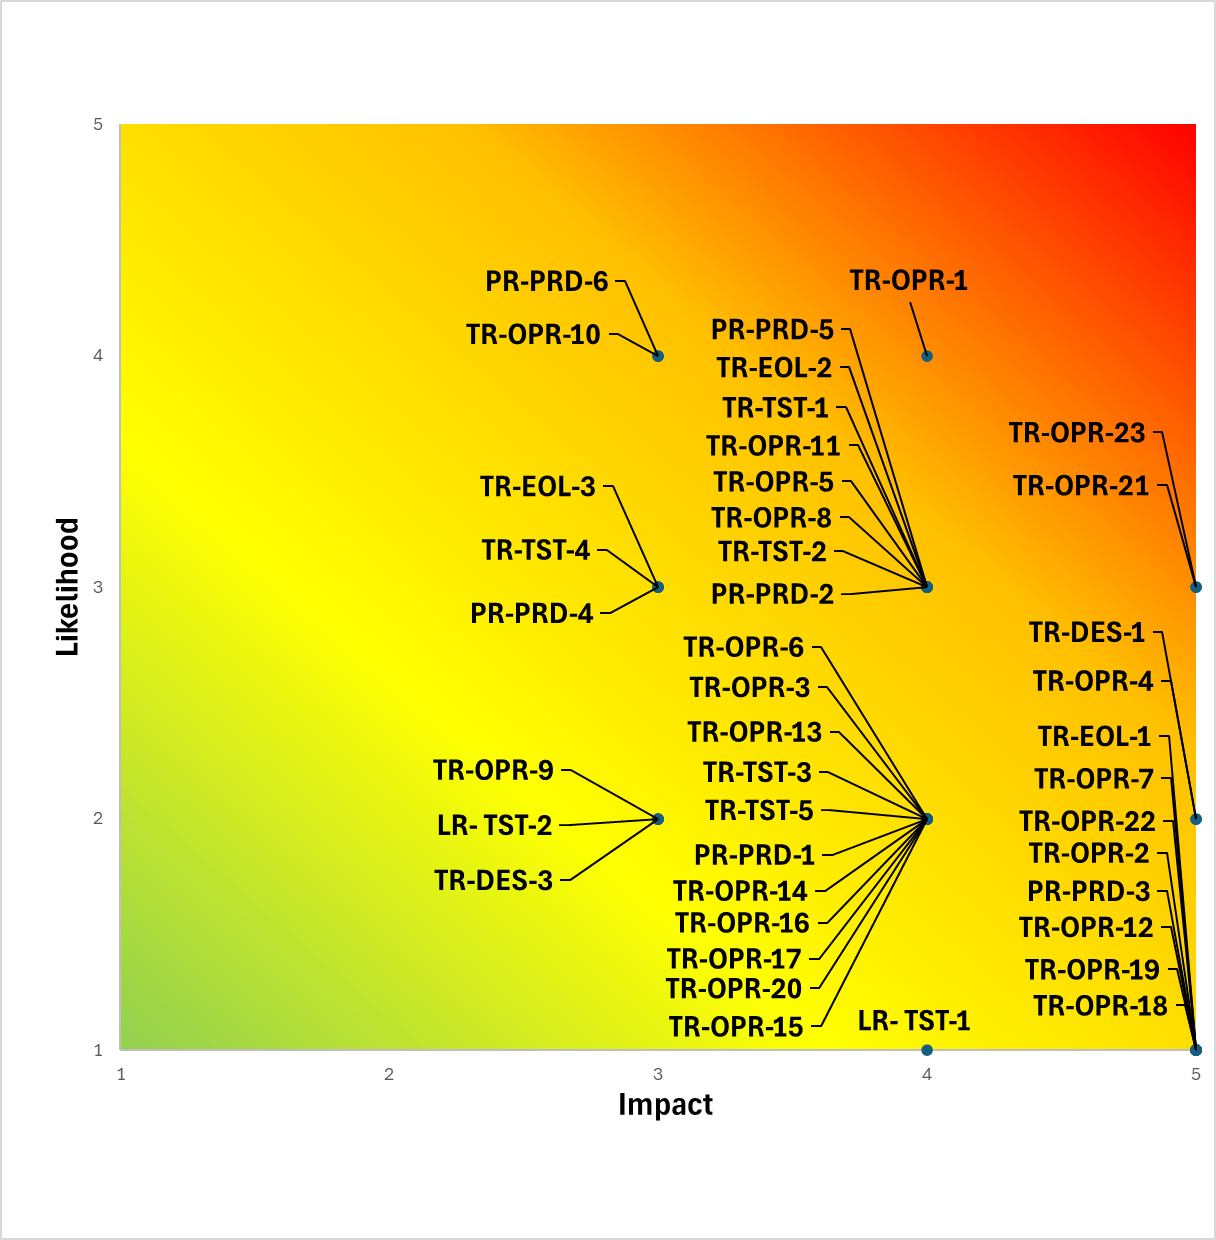
\includegraphics[width=\textwidth]{figures/AE3200 Risk map 1.jpg}
    \caption{Unmitigated risk map}
    \label{fig:risk_unm_tech}
  \end{subfigure}
  \hfill
  \begin{subfigure}[b]{0.45\textwidth} 
    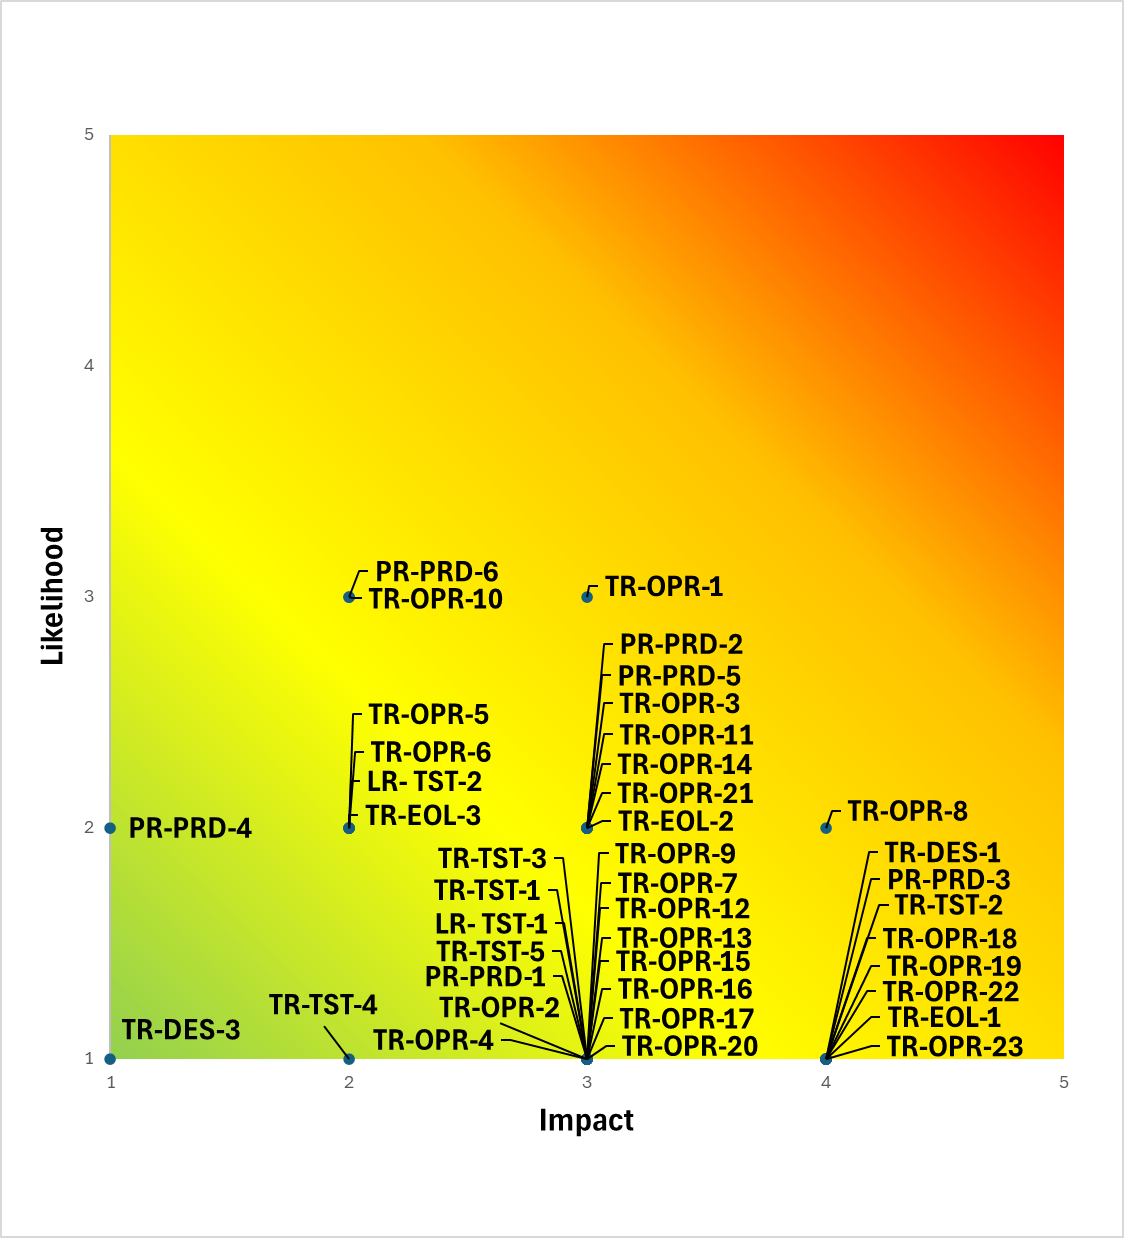
\includegraphics[width=\textwidth]{figures/AE3200 Risk map 2.jpg}
    \caption{Mitigated risk map}
    \label{fig:risk_mit_tech}
  \end{subfigure}
  \caption{Technical risk maps}
  \label{fig:Risk_map}
\end{figure}


\Cref{fig:Risk_map} clearly illustrates the shift in the impact and likelihood risks to more acceptable levels.
Therefore, the risk mitigation and contingency plans that are presented in \Cref{tab:mit_risk_final} greatly benefit the risk analysis.
One can conclude that the risks that should be monitored the most are TR-OPR-1 and TR-OPR8, as they are still situated in the orange area of the mitigated risk map, representing moderate threats.
However, most risks have been decreased to a low to medium threat level (green and yellow), which is beneficial to the project as this implies less vulnerability to different risk factors.